%!TEX root = ../dokumentation.tex

\chapter{Projektziel}
\todo{Projekt Vision}

\section{Projektanforderungen}
Zur Definition der Projektanforderungen wurden mehrere Usecase-Diagramme erstellt.

Zunächst soll der Benutzer auf einer Übersichtsseite ankommen.
Der Usecase dieser Übersichtsseite ist in der Abbilung~\ref{fig:usecaseOverview} dargestellt.
\begin{figure}
    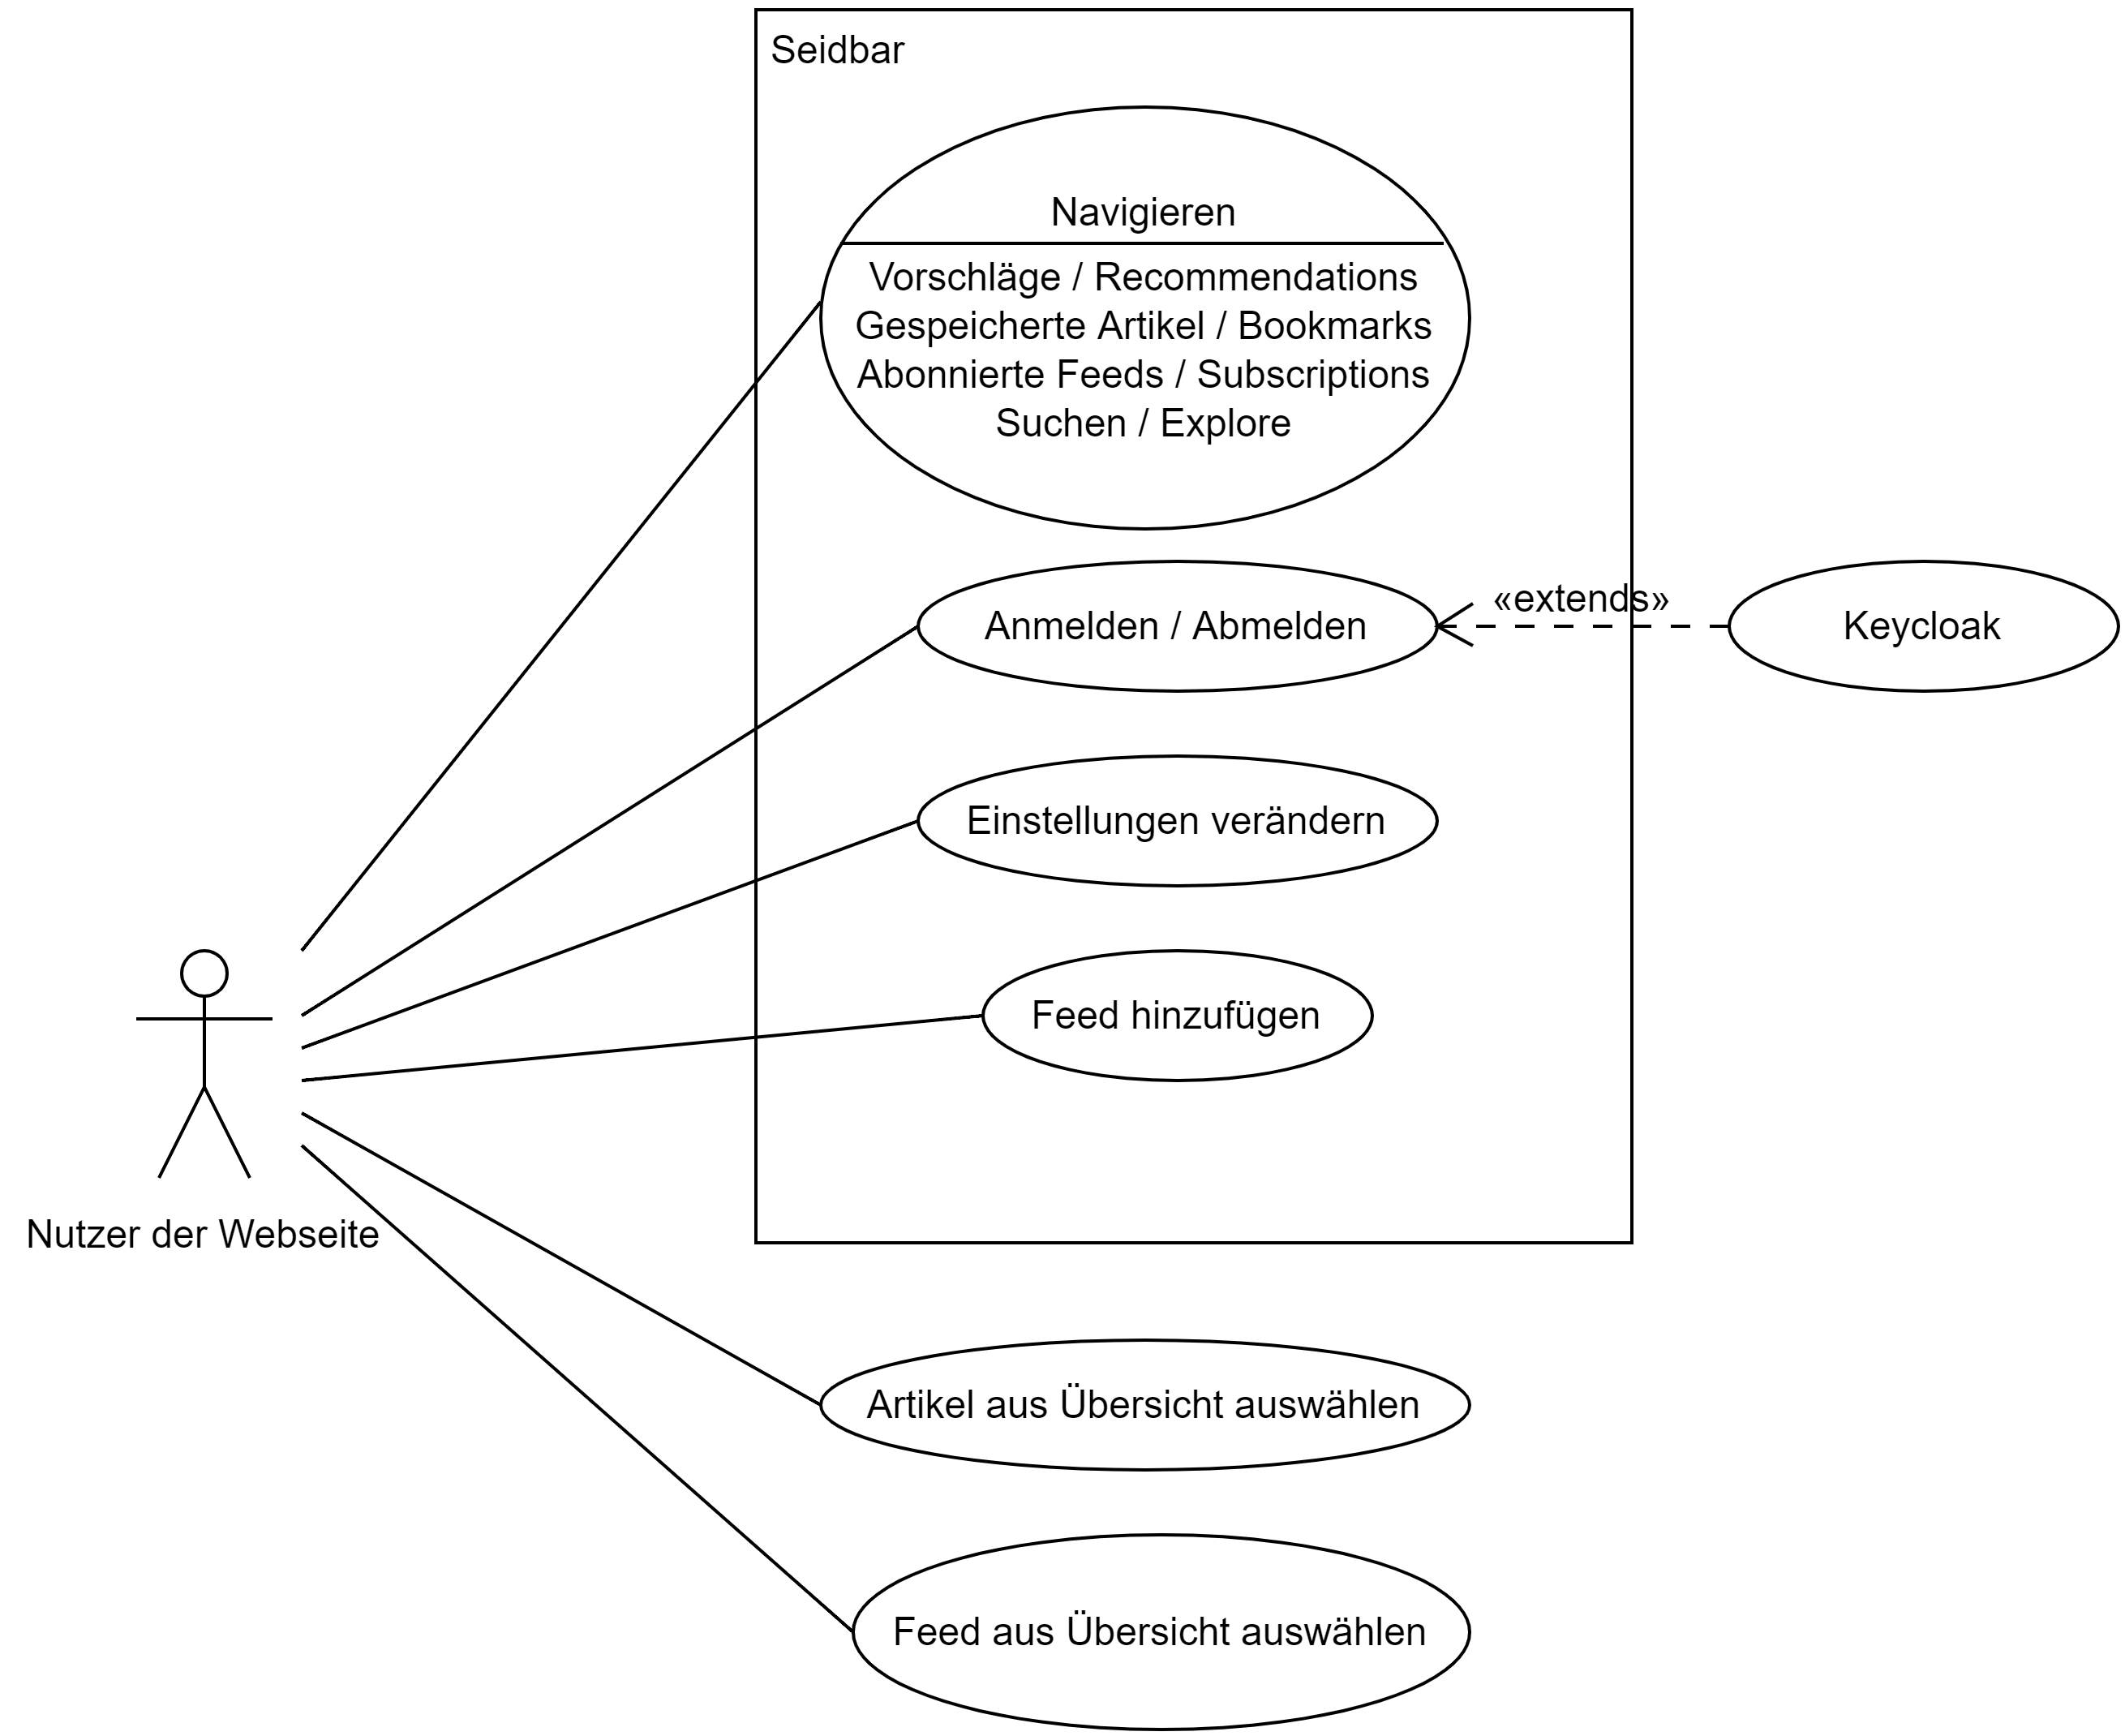
\includegraphics[width=\linewidth]{umlUsecaseOverview.png}
    \caption{Usecase Diagramm der Übersichtsseite}
    \label{fig:usecaseOverview}
\end{figure}
Auf dieser Übersichtsseite werden dem Nutzer verschiedene Feeds und Artikel angezeigt. Mit einem Klick auf einen Feed oder einen Artikel wird
der Nutzer auf eine weitere Seite weitergeleitet mit mehr Möglichkeiten. Außerdem hat der Nutzer auf der Seite über eine Sidebar die Möglichkeit
auf der Seite zu navigieren. Außerdem ist es in der Sidebar möglich seine Usereinstellungen zu ändern, sich an- und abmelden als auch neue Feeds
hinzuzufügen. 
Der Usecase dieser Artikelseite ist in der Abbilung~\ref{fig:usecaseView} dargestellt.
\begin{figure}
    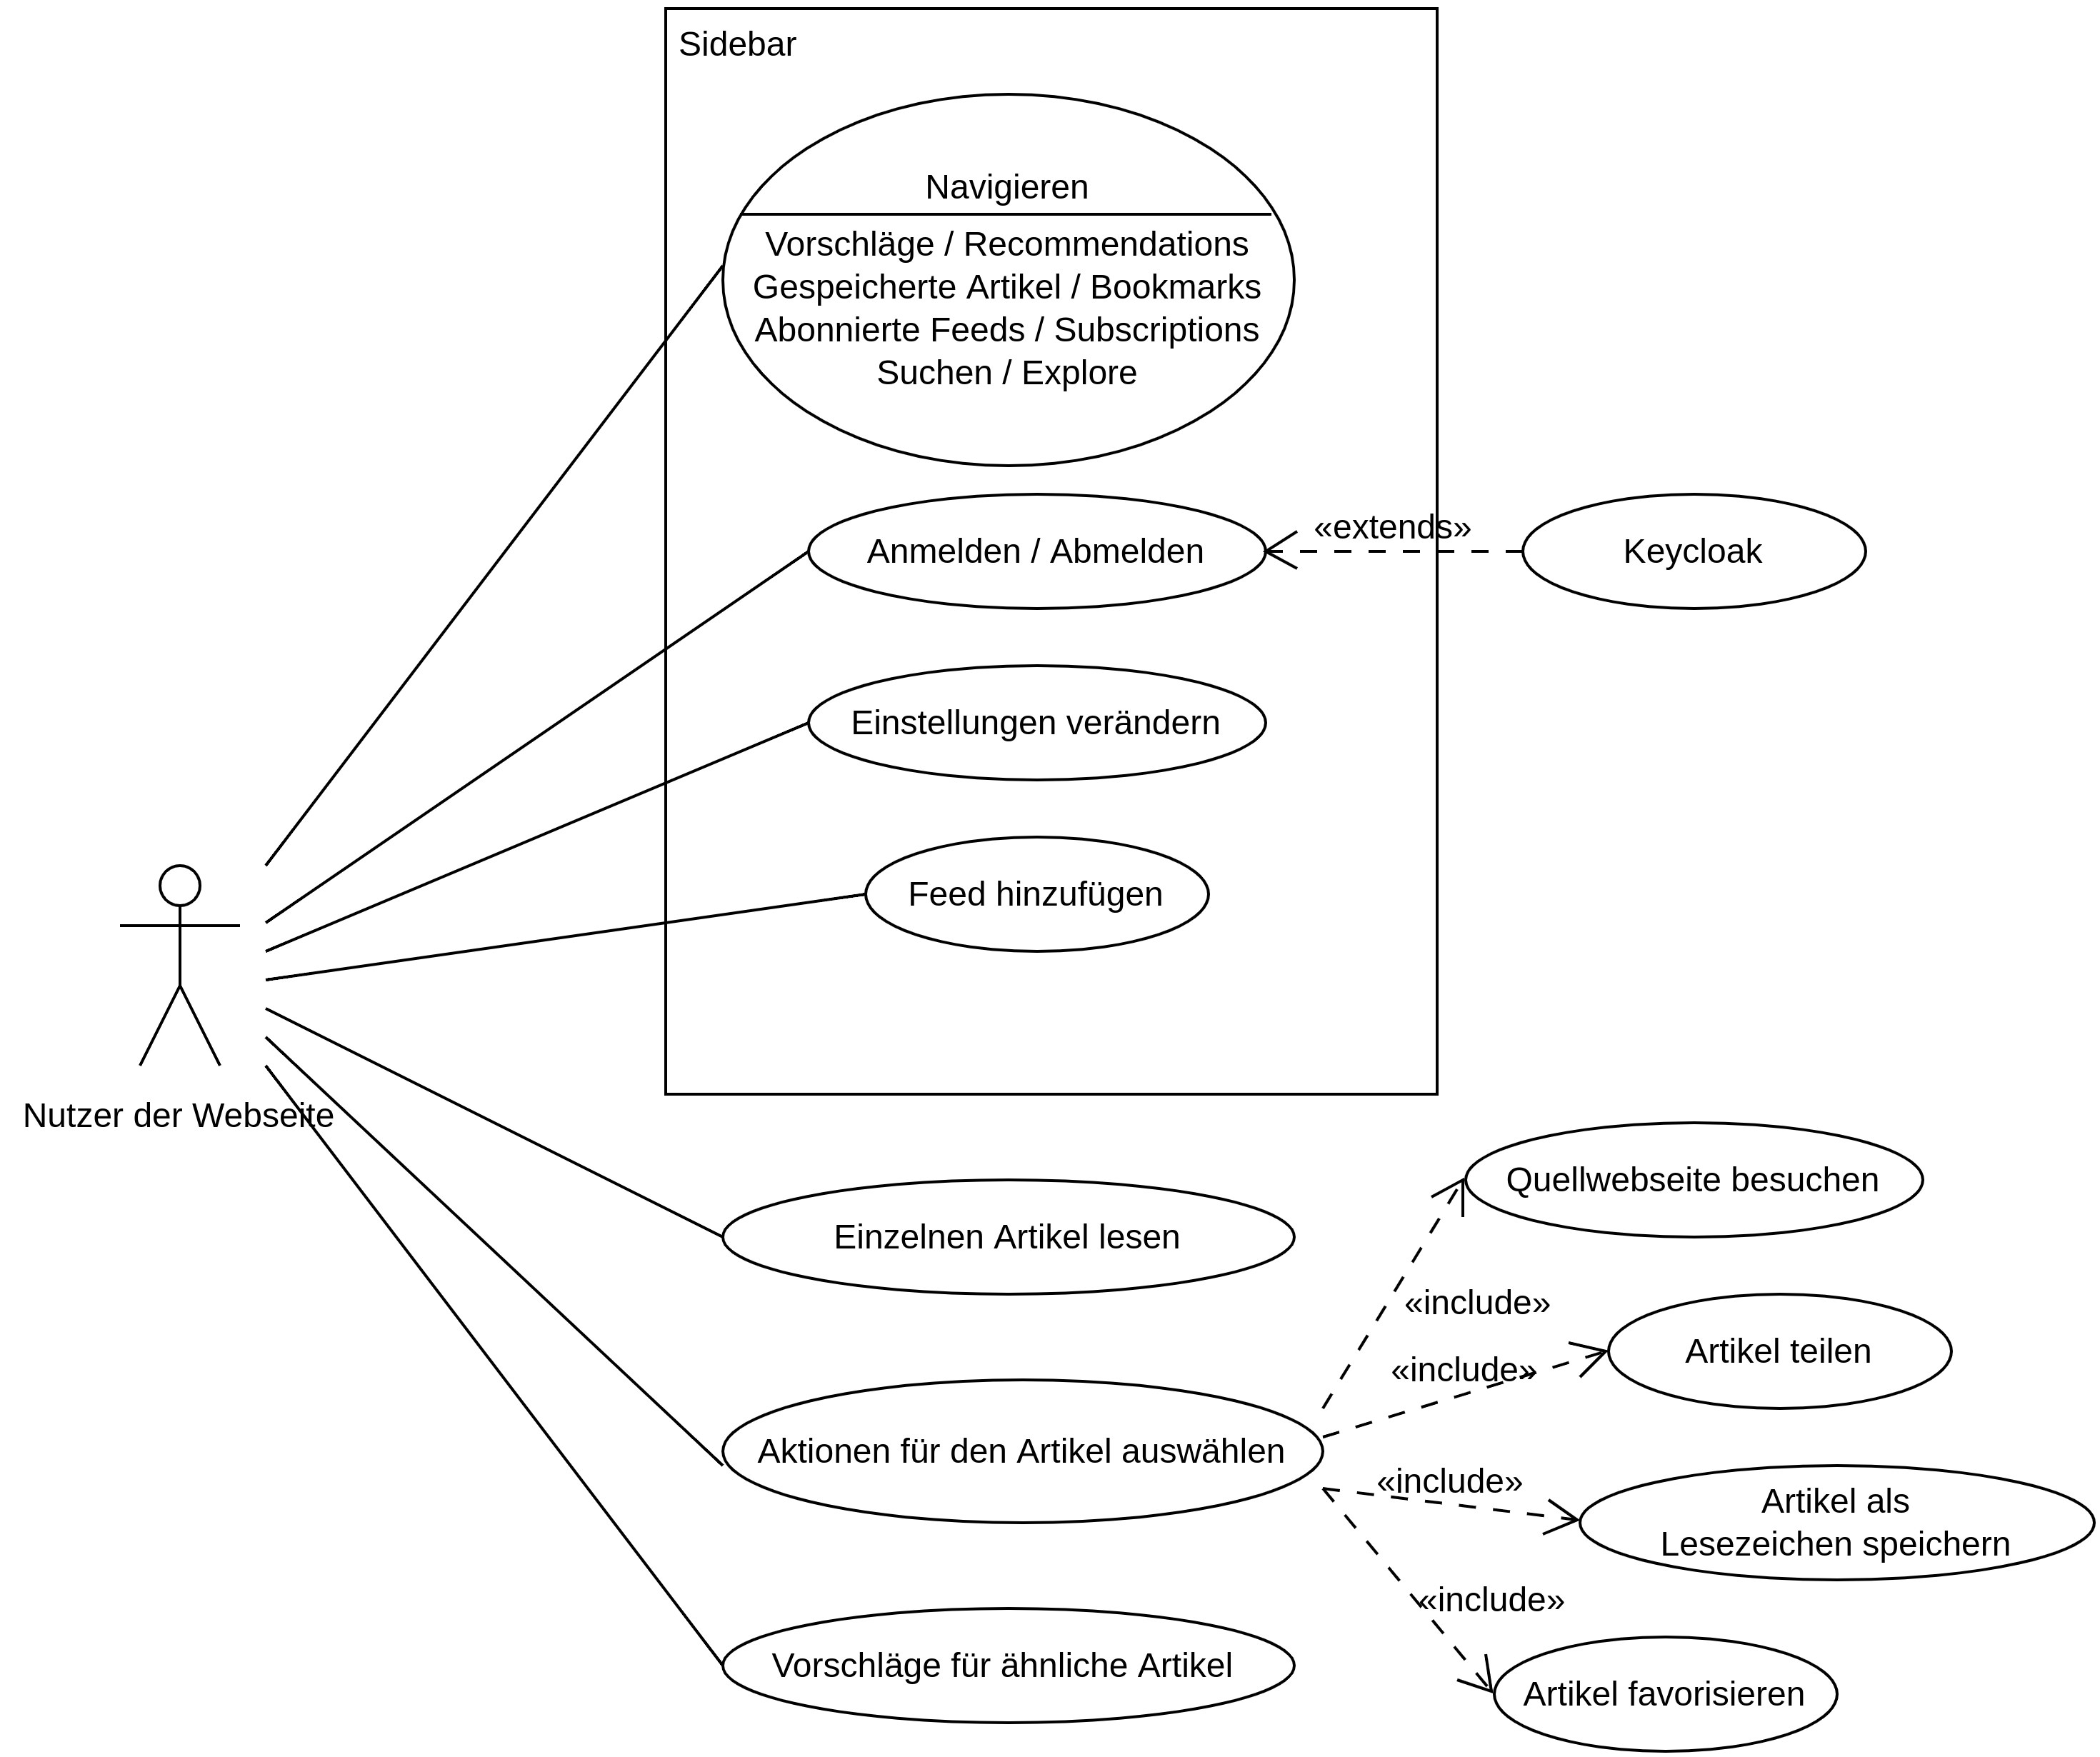
\includegraphics[width=\linewidth]{umlUsecaseView.png}
    \caption{Usecase Diagramm der Artikelseite}
    \label{fig:usecaseView}
\end{figure}
\subsection{Unverzichtbare Ziele}

\subsection{Erreichbare Ziele}

\subsection{Mögliche weiteren Ziele}

\section{Anfängliche Software Architektur}
\todo{Services etc beschreiben}
\todo{Software Auswahl beschreiben (express, angular)}
